\documentclass[tikz,border=8pt]{standalone}
\usepackage{amsmath}
\usetikzlibrary{arrows.meta}

\begin{document}
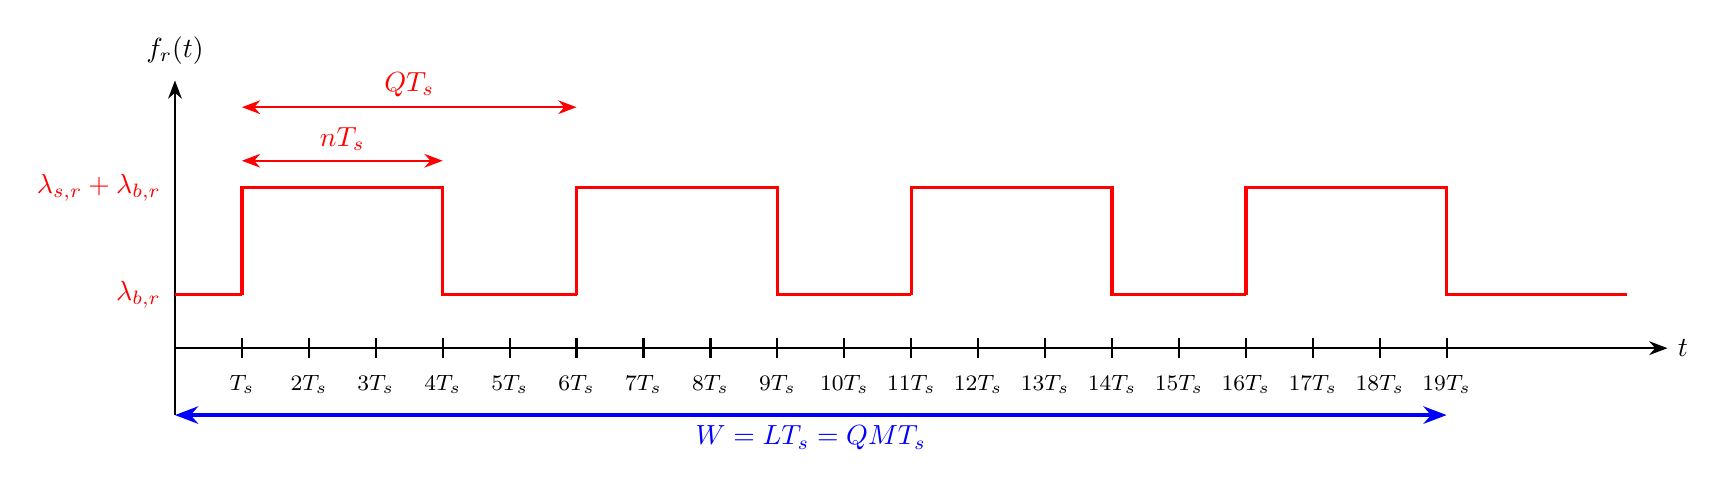
\begin{tikzpicture}[>=Stealth, thick, x=0.85cm, y=0.85cm]
  %================= Parameters (edit these) =================
  \def\Ts{1}     % tick spacing (visual)
  \def\Q{5}      % period length in units of T_s
  \def\n{3}      % ON-time length in units of T_s (nT_s)
  \def\K{4}      % number of periods to draw
  % vertical levels
  \def\ybase{0.8}         % \lambda_{b,r}
  \def\ytop{2.4}          % \lambda_{s,r}+\lambda_{b,r}
  % axis window
  \def\xleft{\Ts}         % left margin
  \pgfmathsetmacro{\xright}{\xleft+\K*\Q} % right end of pulses
  \def\ymin{-1.5}
  \def\ymax{4.0}
  %================= Axes =================
  \draw[->] (0,0) -- (\xright+1.3,0) node[ right] {$t$};
  \draw[->] (0,\ymin+0.5) -- (0,\ymax) node[above=2pt] {$f_r(t)$};

  %================= Pulse train =================
  % start with a short baseline from the left
  \draw[very thick, red] (\xleft-\Ts,\ybase) -- (\xleft,\ybase);
  % draw each period: baseline -> up -> high -> down -> baseline
  \foreach \k in {0,...,\numexpr\K-1\relax}{
    \pgfmathsetmacro{\xs}{\xleft+\k*\Q}
    \draw[very thick, red]
      (\xs,\ybase) -- (\xs,\ytop) -- (\xs+\n,\ytop) -- (\xs+\n,\ybase) -- (\xs+\Q,\ybase);
  }
  % trailing baseline
  \draw[very thick, red] (\xright,\ybase) -- (\xright+0.7,\ybase);

  %================= Level labels =================
  \node[red, left=5pt] at (0.15,\ybase) {$\lambda_{b,r}$};
  \node[red, left=5pt] at (0.15,\ytop) {$\lambda_{s,r}+\lambda_{b,r}$};

  %================= nT_s and QT_s spans (above first period) =================
  \draw[<->, red] (\xleft,\ytop+1.2) -- node[above, red] {$QT_s$} (\xleft+\Q,\ytop+1.2);
  \draw[<->, red] (\xleft,\ytop+0.4) -- node[above, red] {$nT_s$} (\xleft+\n,\ytop+0.4);

  %================= Ticks every T_s with labels T_s, 2T_s, ... =================
  \def\N{19}
  \foreach \i in {1,...,\N}{
    \pgfmathsetmacro{\x}{\i*\Ts}
    \draw (\x,0.15) -- (\x,-0.15);
    \node[below,font=\footnotesize] at (\x,-0.25) {$\ifnum\i=1 T_s\else \i T_s\fi$};
  }

  %================= Long blue span: W = L T_s = Q M T_s =================
  \draw[<->, blue, very thick]
    (0, \ymin+0.5) -- node[below, blue] {$W = L T_s = Q M T_s$} (19*\Ts,\ymin+0.5);

\end{tikzpicture}
\end{document}
